\chapter{Supplementary materials for \autoref{chap:CMZ}}
\section{Materials and methods}
\subsection{Zebrafish husbandry}
Zebrafish husbandry was performed as described in \autoref{ssec:husbandry}.

\subsection{Immunohistochemistry}

\subsection{Confocal micrograph acquisition and processing}

\subsection{Estimation of overall CMZ population and retinal volume}

\subsection{Monte Carlo estimation of CMZ population and retinal volume rates of change}

\subsection{Evidence estimation by Galilean Monte Carlo nested sampling}

\subsection{Evidence estimation by Empirical Bayes linear regression}

\subsection{Simulation of phased CMZ activity by systems of difference equations}

\subsection{Slice model simulations of phased CMZ activity}

\subsection{Estimation of posterior distributions of phase model parameters}

\section{Supplementary Figures}

\begin{figure}[!h]
    \makebox[\textwidth][c]{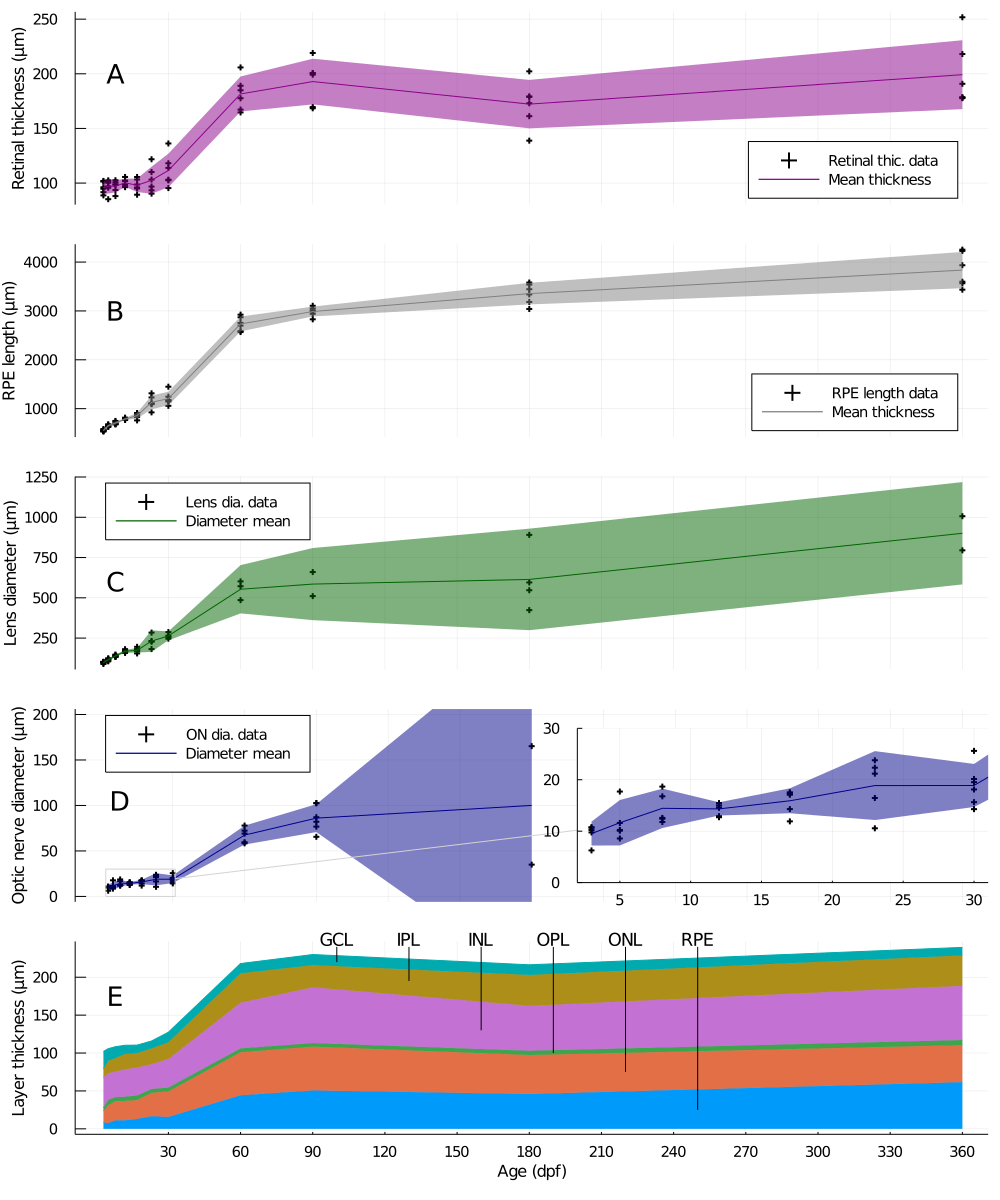
\includegraphics[width=1.2\textwidth]{cmz/morphology.png}}    
    \caption{{\bf Developmental progression of naso-temporal population asymmetry in the CMZ.}}
    \label{morphology}
\end{figure}

\begin{figure}[!h]
    \makebox[\textwidth][c]{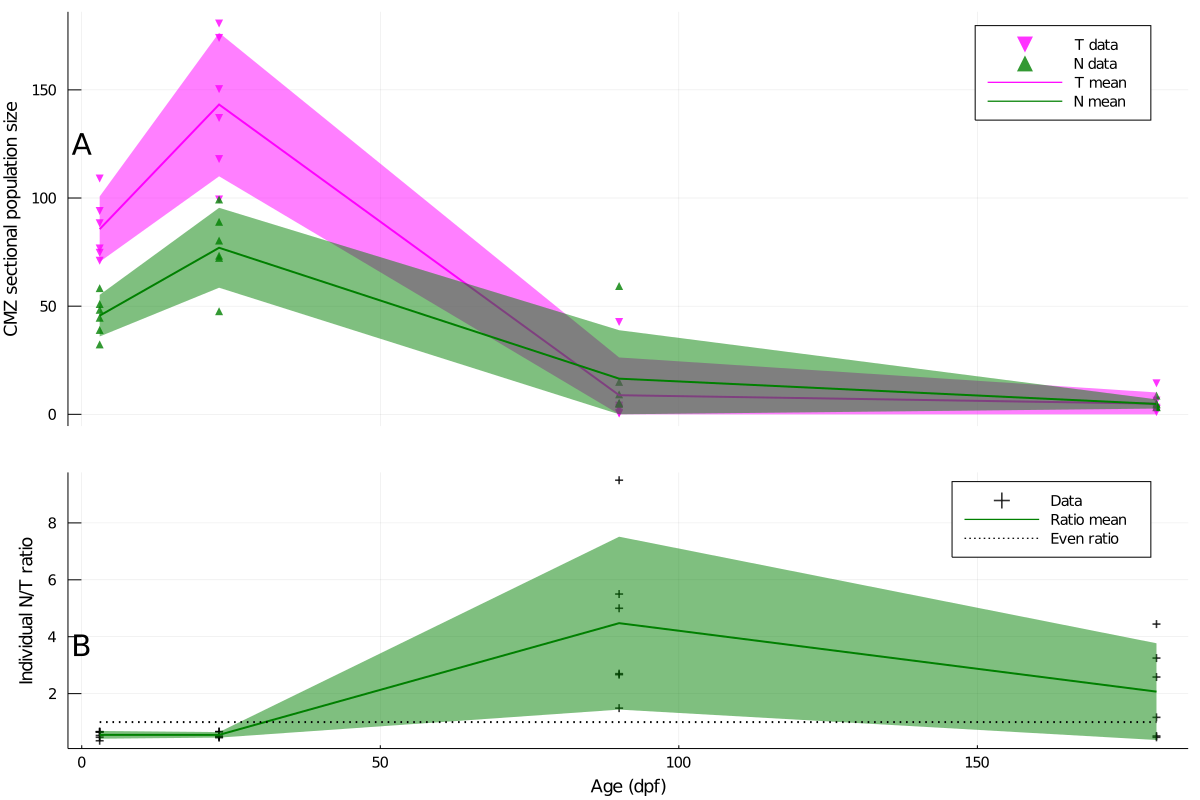
\includegraphics[width=1.2\textwidth]{cmz/NTontology.png}}    
    \caption{{\bf Developmental progression of naso-temporal population asymmetry in the CMZ.}}
    Marginal posterior distribution of mean nasal (N) and temporal (T) population size in 14$\mu$m transverse cryosections (panel A) or intra-individual N/T count asymmetry ratio (panel B), $\pm 95\%$ credible interval, n=6 animals per age. Data points represent mean counts from three central sections of an experimental animal's eye. 
    \label{NTontology}
\end{figure}


\begin{figure}[!h]
    \makebox[\textwidth][c]{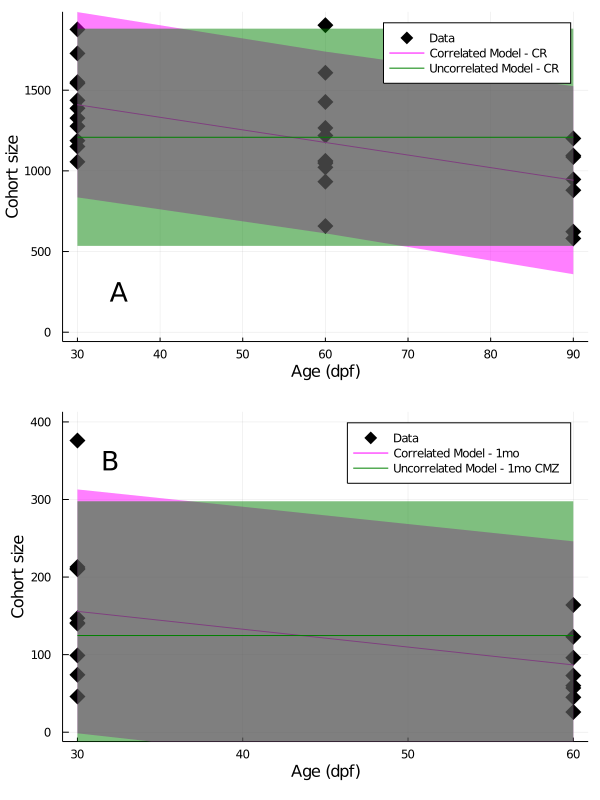
\includegraphics[width=.7\textwidth]{cmz/a27linreg.png}}    
    \caption{{\bf Linear regressions of temporally correlated and uncorrelated models of central retinal and 30dpf CMZ-contributed cohorts}}
    \label{a27linreg}
\end{figure}


\begin{figure}[!h]
    \makebox[\textwidth][c]{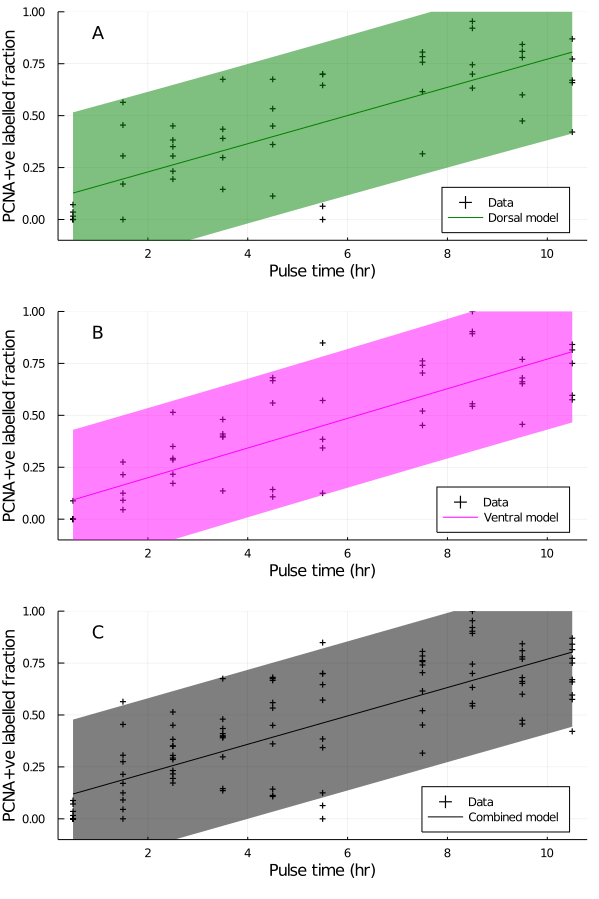
\includegraphics[width=.7\textwidth]{cmz/3ddvlinreg.png}}    
    \caption{{\bf Linear regressions performed on cumulative labelling data from dorsal, ventral, and combined CMZ sectional populations}}
    \label{cumEdUlinreg}
\end{figure}


\begin{figure}[!h]
    \makebox[\textwidth][c]{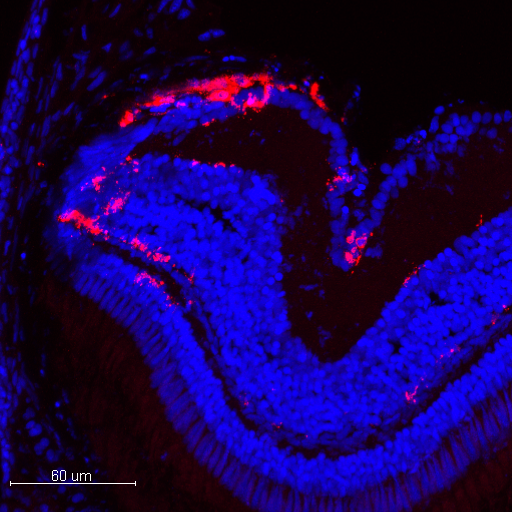
\includegraphics[width=.6\textwidth]{cmz/4C4 distribution.png}}    
    \caption{{\bf 4C4+ microglia are associated with the CMZ}}
    Representative maximum intensity projection from confocal micrographs of 14\si{\micro\metre} coronal cryosections through 90dpf zebrafish eyes.
    
    Blue: Hoechst 33258 nuclear counterstain. Red: Microglia labelled with 4C4 antibody. Note extensive presence of 4C4+ microglia around the peripheral CMZ.
    \label{4C4micrograph}
\end{figure}

\FloatBarrier

\section{Evidence calculations for models of layer and lineage contribution}
\FloatBarrier

\begin{table}[!ht]
    \caption{Evidence for Normal vs. Log-Normal models of layer and lineage contribution}
    \begin{tabular}{|l|l|l|l|l|l|l|} 
        \hline
        {\bf Layer} & {\bf Marker} & {\bf Cell type} & {\bf $\mathcal{N}$ logZ} & {\bf Log-$\mathcal{N}$ logZ} & {\bf logZR} & {\bf $\sigma$ sign.}\\ \hline \hline
        GCL & Cohort & All GCL cells & {\bf -189.0 ± 1.4} & -193.5 ± 1.9 & -4.5 ± 2.4 & 1.9\\ \hline \hline
        GCL & Isl2b & RGC & {\bf -74.5 ± 1.0} & -98.68 ± 0.24 & -24.2 ± 1.1 & -22.74\\ \hline
        GCL & Pax6 & Displaced am. & -101.93 ± 0.96 & {\bf -77.87 ± 0.27} & 24.06 ± 1.0 & 24.2\\ \hline
        GCL & Isl2b/Pax6 & RGC subtype & {\bf -97.9 ± 1.0} & -113.4 ± 0.74 & -15.5 ± 1.3 & 12.4\\ \hline \hline
        INL & Cohort & All INL cells & {\bf -184.0 ± 1.4} & -474.5 ± 2.7 & -290.4 ± 3.1 & 94.0\\ \hline \hline
        INL & Pax6 & Amacrine cell & {\bf -36.83 ± 0.88} & -65.43 ± 0.24 & -28.6 ± 0.92 & 31.3\\ \hline
        INL & PKC$\beta$ & Bipolar cell & -37.83 ± 0.2 & {\bf -0.77 ± 0.67} & 37.06 ± 0.7 & 53.1\\ \hline
        INL & GS & M\"{u}ller glia & -25.11 ± 0.2 & {\bf 6.7 ± 1.1} & 31.8 ± 1.1 & 29.2\\ \hline
        INL & HM & Horizontal cell & -31.97 ± 0.27 & {\bf 6.73 ± 0.61} & 38.7 ± 0.66 & 58.4\\ \hline \hline
        ONL & Cohort & All ONL cells & {\bf -201.0 ± 1.5} & -335.3 ± 1.5 & -134.2 ± 2.1 & 63.7\\ \hline \hline
        ONL & Zpr1 & Double cones & {\bf -93.7 ± 1.4} & -146.91 ± 0.8 & -53.2 ± 1.6 & 33.2\\ \hline
    \end{tabular}
   
    \begin{flushleft}logZ: logarithm of p(D), the marginal likelihood of the data, or model evidence.  Largest evidence values bolded. logZR: evidence ratio; positive values in favour of stable model.
    \end{flushleft}
    \label{lineage_nlnev}
\end{table}

\begin{table}[!ht]
    \caption{Evidence for combined vs. split models of layer and lineage contribution across the dorso-ventral axis}
    \begin{tabular}{|l|l|l|l|l|l|l|} 
        \hline
        {\bf Layer} & {\bf Marker} & {\bf Cell type} & {\bf Combined D-V logZ} & {\bf Split D-V logZ} & {\bf logZR} & {\bf $\sigma$ sign.}\\ \hline \hline
        GCL & Cohort & All GCL cells & {\bf -41.64 ± 0.63} & -186.04 ± 0.39 & 144.4 ± 0.74 & 194.1\\ \hline \hline
        GCL & Isl2b & RGC & {\bf -47.58 ± 0.84} & -69.6 ± 1.0 & 22.0 ± 1.3 & 16.7\\ \hline
        GCL & Pax6 & Displaced am. & {\bf -32.65 ± 0.68} & -54.3 ± 1.5 & 21.7 ± 1.6 & 13.4\\ \hline
        GCL & Isl2b/Pax6 & RGC subtype & {\bf -40.94 ± 0.77} & -90.3 ± 1.2 & 49.3 ± 1.4 & 35.5\\ \hline \hline
        INL & Cohort & All INL cells & {\bf -83.5 ± 1.0} & -124.2 ± 1.1 & 40.7 ± 1.5 & 26.5\\ \hline \hline
        INL & Pax6 & Amacrine cell & {\bf -15.66 ± 0.041} & -56.15 ± 0.91 & 40.49 ± 0.91 & 44.4\\ \hline
        INL & PKC$\beta$ & Bipolar cell & {\bf -10.52 ± 0.46} & -23.3 ± 1.1 & 12.8 ± 1.2 & 11.1\\ \hline
        INL & GS & M\"{u}ller glia & {\bf 13.69 ± 0.36} & 3.5 ± 2.4 & 10.2 ± 2.4 & 4.2\\ \hline
        INL & HM & Horizontal cell & {\bf 9.81 ± 0.37} & -10.1 ± 1.3 & 19.9 ± 1.4 & 14.4\\ \hline \hline
        ONL & Cohort & All ONL cells & {\bf -73.06 ± 0.84} & -141.3 ± 1.1 & 68.2 ± 1.4 & 48.0\\ \hline \hline
        ONL & Zpr1 & Double cones & {\bf -41.17 ± 0.75} & -63.0 ± 0.89 & 21.8 ± 1.2 & 18.8\\ \hline
    \end{tabular}
\begin{flushleft}logZ: logarithm of p(D), the marginal likelihood of the data, or model evidence.  Largest evidence values bolded. logZR: evidence ratio; positive values in favour of combined model.
\end{flushleft}
\label{lineage_dvev}
\end{table}


\section{Likelihood ratio calculations for Normal and Log-Normal models of layer and lineage contribution}

\begin{table}[!ht]
    \begin{tabular}{|l|l|l|l|l|l|l|} 
        \hline
        {\bf Layer} & {\bf Marker} & {\bf Cell type} & {\bf $\mathcal{N}$ MLE} & {\bf Log-$\mathcal{N}$ MLE} & {\bf lhR}\\ \hline \hline
        GCL & Cohort & All GCL cells & 54.194 & {\bf 55.835} & 1.642\\ \hline
        GCL & Isl2b & RGC & 14.439 & {\bf 19.106} & 4.667\\ \hline
        GCL & Pax6 & Displaced am. &  8.287 & {\bf 11.158} & 2.871\\ \hline
        GCL & Isl2b/Pax6 & RGC subtype & 20.292 & {\bf 28.139} & 7.847\\ \hline
        INL & Cohort & All INL cells & 44.942 & {\bf 45.179} & 0.237\\ \hline
        INL & Pax6 & Amacrine cell & {\bf 23.808} & 23.178 & -0.63\\ \hline
        INL & PKC$\beta$ & Bipolar cell & {\bf 27.243} & 26.119 & -1.124\\ \hline
        INL & GS & M\"{u}ller glia & 30.847 & {\bf 31.818} & 0.97\\ \hline
        INL & HM & Horizontal cell & 27.65 & {\bf 29.431} & 1.78\\ \hline
        ONL & Cohort & All ONL cells & 41.488 & {\bf 43.195} & 1.706\\ \hline
        ONL & Zpr1 & Double cones & 13.256 & {\bf 18.483} & 5.227\\ \hline
    \end{tabular}
   
    \begin{flushleft}logZ: logarithm of p(D), the marginal likelihood of the data, or model evidence.  Largest evidence values bolded. logZR: evidence ratio; positive values in favour of stable model.
    \end{flushleft}
    \label{lineage_lhratio}
\end{table}


